\section{贝叶斯统计推断}


\subsection{贝叶斯推断与后验分布}

\begin{figure}[H]
    \centering
    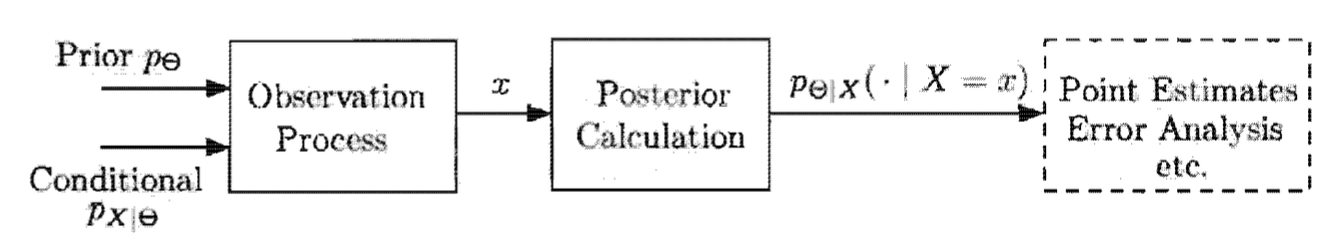
\includegraphics[width=0.8\linewidth]{figs/贝叶斯推断模型.png}
    \caption{贝叶斯推断模型}
    \label{fig:bayesian-inference}
\end{figure}

记感兴趣的未知量为 $\Theta$,并视其为一个随机变量或随机变量的有限集合。我们的目标是基于观测到相关随机变量的值 $X=(X_1,\ldots,X_n)$ 来提取 $\Theta$ 的信息。假定我们已知先验分布 $p_\Theta$ 或 $f_\Theta$,以及条件分布 $p_{X\vert\Theta}$ 或 $f_{X\vert\Theta}$,则贝叶斯推断问题由 $\Theta$ 的后验分布 $p_{\Theta\vert X}$ 或 $f_{\Theta\vert X}$ 完全决定。后验分布可根据贝叶斯公式计算。
% 根据 $\Theta$ 和 $X$ 的离散性和连续性,贝叶斯公式由四种组合方式:
% \begin{gather*}
% p_{\Theta\vert X}(\theta\vert x)=\frac{p_\Theta(\theta)p_{X\vert\Theta}(x\vert\theta)}{\sum_{\theta'}p_\Theta(\theta')p_{X\vert\Theta}(x\vert\theta')},\qquad\text{$\Theta$ 离散,$X$ 离散}\\
% p_{\Theta\vert X}(\theta\vert x)=\frac{p_\Theta(\theta)f_{X\vert\Theta}(x\vert\theta)}{\sum_{\theta'}p_\Theta(\theta')f_{X\vert\Theta}(x\vert\theta')},\qquad\text{$\Theta$ 离散,$X$ 连续}\\
% f_{\Theta\vert X}(\theta\vert x)=\frac{f_\Theta(\theta)p_{X\vert\Theta}(x\vert\theta)}{\int f_\Theta(\theta')p_{X\vert\Theta}(x\vert\theta')\mathrm d\theta'},\qquad\text{$\Theta$ 连续,$X$ 离散}\\
% f_{\Theta\vert X}(\theta\vert x)=\frac{f_\Theta(\theta)f_{X\vert\Theta}(x\vert\theta)}{\int f_\Theta(\theta')f_{X\vert\Theta}(x\vert\theta')\mathrm d\theta'},\qquad\text{$\Theta$ 连续,$X$ 连续}
% \end{gather*}

\begin{example}[正态随机变量公共均值的推断]
\label{ex:normal-mean-infer}
设随机变量观测值 $X=(X_1,\ldots,X_n)$ 具有相同的未知均值。假设在给定均值的条件下,$X_i$ 是正态的,且相互独立,方差分别为 $\sigma_1^2,\ldots,\sigma_n^2$. 又设 $X_i$ 的公共均值为随机变量 $\Theta$,且先验分布为正态分布 $N(x_0,\sigma_0^2)$. 那么:
\begin{gather*}
f_\Theta(\theta)=c_1\cdot\exp\left(-\frac{(\theta-x_0)^2}{2\sigma_0^2}\right)\\
f_{X\vert\Theta}(x\vert\theta)=c_2\cdot\exp\left(-\frac{(x_1-\theta)^2}{2\sigma_1^2}\right)\cdots\exp\left(-\frac{(x_n-\theta)^2}{2\sigma_n^2}\right)
\end{gather*}
其中 $c_1,c_2$ 为常数。根据贝叶斯公式,有:
\begin{align*}
f_{\Theta\vert X}(\theta\vert x)\propto f_\Theta(\theta)f_{X\vert\Theta}(x\vert\theta)\propto\exp\left(-\sum_{i=0}^n\frac{(\theta-x_i)^2}{2\sigma_i^2}\right)\propto\exp\left(-\frac{(\theta-m)^2}{2v}\right)
\end{align*}
其中根据配方可得:
\[
m=\frac{\sum_{i=0}^nx_i/\sigma_i^2}{\sum_{i=0}^n1/\sigma_i^2},\quad v=\frac{1}{\sum_{i=0}^n1/\sigma_i^2}
\]
于是后验概率就是以 $m$ 为均值、$v$ 为方差的正态分布。
\end{example}

\begin{definition}[共轭分布]
在贝叶斯推断中,若先验分布与后验分布是同一个分布族,则先验分布与后验分布被称为共轭分布。
\end{definition}
\begin{com}
例 \ref{ex:normal-mean-infer} 显示正态分布与其自身是共轭分布。这并不是一个普遍的情形,除了正态分布以外,其他常见的与自身共轭的分布有伯努利分布和二项分布。
\end{com}


\subsection{点估计,假设检验,最大后验概率准则}

\paragraph{点估计}
给定 $X$ 的观测值 $x$,贝叶斯推断给出了后验分布 $p_{\Theta\vert X}(\theta\vert x)$ 或 $f_{\Theta\vert X}(\theta\vert x)$. 后验分布包含了 $x$ 提供的所有信息,但有时我们希望得到一个数而不是一个概率分布,这就是点估计。具体而言,点估计指从 $X$ 的观测值中提取一个数 $\hat\theta=g(x)$ 作为对 $\Theta$ 的估计的方法。

\begin{definition}[估计量,估计值]
设 $g$ 是一个关于 $X$ 的函数,则称随机变量 $\hat\Theta=g(X)$ 为估计量。当观测到 $X$ 的值 $x$ 后,则称 $\hat\Theta$ 的取值 $\hat\theta=g(x)$ 为估计值。不同的函数 $g$ 引出不同的估计量。
\end{definition}

\begin{definition}[最大后验概率估计量]
给定 $X$ 的观测值 $x$,选择使得后验概率最大的 $\theta$ 作为估计值,即:
\[
\hat\theta=\max_\theta p_{\Theta\vert X}(\theta\vert x)\;\text{或}\;\max_\theta f_{\Theta\vert X}(\theta\vert x)
\]
\end{definition}

\begin{definition}[条件期望估计量]
给定 $X$ 的观测值 $x$,选择条件期望作为估计值,即:
\[
\hat\theta=\E[\Theta\vert X=x]
\]
\end{definition}
\begin{com}
在下一节中将看到,条件期望估计量其实就是最小均方估计量。
\end{com}

\begin{example}[正态随机变量公共均值的估计量]
\label{ex:normal-mean-estimate}
在例 \ref{ex:normal-mean-infer} 中,我们得到了正态随机变量公共均值 $\Theta$ 的后验分布是以 $m$ 为均值、$v$ 为方差的正态分布,其中:
\[
m=\frac{\sum_{i=0}^nx_i/\sigma_i^2}{\sum_{i=0}^n1/\sigma_i^2},\quad v=\frac{1}{\sum_{i=0}^n1/\sigma_i^2}
\]
由于正态分布的概率密度函数在均值处取最大值,所以最大后验概率估计为:
\[
\hat\theta=m
\]
而正态分布的均值参数正是其期望,因此条件期望估计也为:
\[
\hat\theta=\E[\Theta\vert X=x]=m
\]
因此在该模型中,最大后验概率估计和条件期望估计恰好相同。
\end{example}

\paragraph{假设检验}
在一个假设检验问题中,$\Theta$ 取 $\theta_1,\ldots,\theta_m$ 中的一个值,其中 $m$ 是一个较小的整数(常常是 $m=2$)。称事件 $H_i=\{\Theta=\theta_i\}$ 为第 $i$ 个假设。观测到 $X$ 的取值 $x$ 后,我们希望依据某种准则选出一个最“合理”的假设。

\begin{definition}[假设检验的最大后验概率准则]
给定观测值 $x$,最大后验概率准则选择使得后验概率 $\Pb(\Theta=\theta_i\vert X=x)$ 最大的假设 $H_i$:
\[
\arg\max_i\;\Pb(\Theta=\theta_i\vert X=x)
\]
根据贝叶斯公式,这等价于:
\begin{gather*}
    \arg\max_i\;p_\Theta(\theta_i)p_{X\vert\Theta}(x\vert\theta_i),\quad\text{$X$ 离散}\\
    \arg\max_i\;p_\Theta(\theta_i)f_{X\vert\Theta}(x\vert\theta_i),\quad\text{$X$ 连续}
\end{gather*}
\end{definition}
\begin{com}
对任意观测值 $x$,最大后验概率准则是错误率最小的决策准则。
\end{com}


\subsection{贝叶斯最小均方估计}

\begin{theorem}[最小均方估计——无观测值情形]
\label{thm:lms-not-given-x}
考虑在没有观测值的情况下,用常数 $\hat\theta$ 去估计 $\Theta$,则使得均方误差 $\E[(\Theta-\hat\theta)^2]$ 最小的估计为:
\[\hat\theta=\E\Theta\]
换句话说,有:
\[
\E[(\Theta-\E\Theta)^2]\leq\E[(\Theta-\hat\theta)^2],\quad\forall\,\hat\theta
\]
\end{theorem}
\begin{proof}
对任何估计 $\hat\theta$,有均方误差:
\[
\E[(\Theta-\hat\theta)^2]=\var(\Theta-\hat\theta)+(\E[\Theta-\hat\theta])^2=\var(\Theta)+(\E\Theta-\hat\theta)^2
\]
由于 $\var(\Theta)$ 与 $\hat\theta$ 无关,故当 $(\E\Theta-\hat\theta)^2$ 最小时均方误差最小,也即 $\hat\theta=\E\Theta$.
\end{proof}

\begin{theorem}[最小均方估计——给定观测值情形]
\label{thm:lms-given-x}
设给定观测值 $x$,则使得均方误差 $\E[(\Theta-\hat\theta)^2\vert X=x]$ 最小的估计为条件期望估计:
\[\hat\theta=\E[\Theta\vert X=x]\]
换句话说,有:
\[
\E[(\Theta-\E[\Theta\vert X=x])^2\vert X=x]\leq\E[(\Theta-\hat\theta)^2\vert X=x],\quad\forall\,\hat\theta
\]
\end{theorem}
\begin{proof}
在定理 \ref{thm:lms-not-given-x} 的证明中加入 $X=x$ 的条件即可。
\end{proof}

\begin{theorem}[最小均方估计——总体情形]
\label{thm:lms-overall}
总体上,设估计量为 $\hat\Theta$,则使得均方误差 $\E[(\Theta-\hat\Theta)^2]$ 最小的估计量为:
\[
\hat\Theta=\E[\Theta\vert X]
\]
换句话说,有:
\[
\E[(\Theta-\E[\Theta\vert X])^2]\leq \E[(\Theta-\hat\Theta)^2],\quad\forall\,\hat\Theta=g(X)
\]
\end{theorem}
\begin{proof}
对于任意给定 $X$ 的取值 $x$,$\hat\theta=g(x)$ 是一个数,因此:
\[
\E[(\Theta-\E[\Theta\vert X=x])^2\vert X=x]\leq\E[(\Theta-g(x))^2\vert X=x]
\]
根据 $x$ 的任意性,有:
\[
\E[(\Theta-\E[\Theta\vert X])^2\vert X]\leq\E[(\Theta-g(X))^2\vert X]
\]
根据全期望公式,两边取期望得:
\[
\E[(\Theta-\E[\Theta\vert X])^2]\leq\E[(\Theta-g(X))^2]
\]
\end{proof}

\begin{property}
将最小均方估计和估计误差分别记为:
\[
\hat\Theta=\E[\Theta\vert X],\quad\tilde\Theta=\hat\Theta-\Theta
\]
在 \ref{sec:cond-e-cond-var} 节中已经推导了一些性质,这里列举如下:
\begin{itemize}
    \item $\tilde\Theta$ 是无偏的,它的条件期望和非条件期望都是 0:
    $\E[\tilde\Theta]=0,\;\E[\tilde\Theta\vert X=x]=0,\,\forall\,x$
    \item 估计误差 $\tilde\Theta$ 与估计量 $\hat\Theta$ 不相关:
    $\var(\hat\Theta,\tilde\Theta)=0$
    \item $\Theta$ 的方差可以分解为:
    $\var(\Theta)=\var(\hat\Theta)+\var(\tilde\Theta)$
\end{itemize}
\end{property}

\begin{theorem}[推广到多观测情形]
设有多个观测量 $X_1,\ldots,X_n$,则最小均方估计为:
\[
\hat\Theta=\E[\Theta\vert X_1,\ldots,X_n]
\]
换句话说,有:
\[
\E[(\Theta-\E[\Theta\vert X_1,\ldots,X_n])^2]\leq\E[(\Theta-\hat\Theta)^2],\quad\forall\,\hat\Theta=g(X_1,\ldots,X_n)
\]
\end{theorem}

\subsection{贝叶斯线性最小均方估计}
\label{sec:bayesian-lms}

\begin{definition}[线性估计量]
限定 $g$ 是关于 $X$ 的线性函数 $g(X)=aX+b$,称随机变量:
\[\hat\Theta=g(X)=aX+b\]
为线性估计量。进一步地,若有多个观测量 $X_1,\ldots,X_n$,则线性估计量的形式为:
\[\hat\Theta=a_1X_1+\cdots+a_nX_n+b\]
\end{definition}

\begin{theorem}[线性最小均方估计]
\label{thm:linear-lms-estimate}
基于 $X$ 的 $\Theta$ 的线性最小均方估计是:
\[
\hat\Theta=\E\Theta+\frac{\cov(\Theta,X)}{\var(X)}(X-\E X)=\E\Theta+\rho\frac{\sigma_\Theta}{\sigma_X}(X-\E X)
\]
其中 $\rho=\dfrac{\cov(\Theta,X)}{\sigma_\Theta\sigma_X}$ 是相关系数,此时所得均方误差为:
\[
\E[(\Theta-aX-b)^2]=(1-\rho^2)\sigma_\Theta^2
\]
\end{theorem}
\begin{proof}
假设固定 $a$,则问题等价于选择常数 $b$ 来估计随机变量 $\Theta-aX$. 根据之前的讨论,最优解为:
\[
b=\E[\Theta-aX]=\E\Theta-a\E X
\]
因此问题转化为:
\[
\min_a\;\E[(\Theta-aX-\E[\Theta-aX])^2]=\var(\Theta-aX)
\]
打开方差:
\[
\var(\Theta-aX)=\var(\Theta)+\var(aX)-2\cov(\Theta,aX)=\sigma_\Theta^2+a^2\sigma_X^2-2a\rho\sigma_\Theta\sigma_X
\]
这是关于 $a$ 的二次函数,最小值在顶点处取得:
\[
a=\frac{\rho\sigma_\Theta\sigma_X}{\sigma_X^2}=\rho\frac{\sigma_\Theta}{\sigma_X}
\]
因此线性最小均方估计为:
\[
\hat\Theta=aX+b=aX+\E\Theta-a\E X=\E\Theta+\rho\frac{\sigma_\Theta}{\sigma_X}(X-\E X)
\]
且估计误差为:
\[
\var(\Theta-aX)=\sigma_\Theta^2+a^2\sigma_X^2-2a\rho\sigma_\Theta\sigma_X=\sigma_\Theta^2+\rho^2\sigma_\Theta^2-2\rho^2\sigma_\Theta^2=(1-\rho^2)\sigma_\Theta^2
\]
\end{proof}
\begin{remark}
直观上,估计量以 $\E\Theta$ 为基础,通过 $X-\E X$ 的取值来调整。例如,不妨假设 $\rho>0$,则当观测到比 $\E X$ 更大的 $X$ 取值后,我们对 $\Theta$ 的估计也就相应地提高。另外,当 $|\rho|$ 接近 1 时,$X$ 和 $\Theta$ 高度相关,了解 $X$ 将帮助我们准确地估计 $\Theta$,因此均方误差较小。
\end{remark}

\begin{example}[正态随机变量公共均值的估计量-续]
在例 \ref{ex:normal-mean-estimate} 中,我们得到正态随机变量公共均值的最小均方估计(条件期望估计)为:
\[
\hat\theta=\E[\Theta\vert X=x]=m=\frac{\sum_{i=0}^nx_i/\sigma_i^2}{\sum_{i=0}^n1/\sigma_i^2}
\]
进一步,注意到上式是观测值 $x_1,\ldots,x_n$ 的线性组合,因此它其实也是线性最小均方估计。也即,在该模型中,最大后验概率估计、最小均方估计和线性最小均方估计恰好都是相同的。
\end{example}
